\section{Task 1} \label{sec:Task1}

Die Modellierung eines Leistungselektronik-Wandlers ist ein essenzieller Schritt zur Analyse und Regelung des Systems. In diesem Kapitel wird zunächst die theoretische Grundlage für die Modellbildung erörtert. Anschließend wird das erstellte Modell detailliert beschrieben, einschließlich der verwendeten Komponenten und Parameter. Besondere Aufmerksamkeit wird auf die Wahl der Modellstruktur und deren Einfluss auf das dynamische Verhalten des Systems gelegt. Darüber hinaus werden mögliche Vereinfachungen diskutiert, um eine effiziente Implementierung des Reglers zu ermöglichen. (Siehe Abbildung: \ref{fig:ControllerSoft} und \ref{fig:SystemSoft})

Ein besonderer Fokus lag auf der Auslegung eines PID-Reglers für das System. Verschiedene Methoden zur Bestimmung der Reglerparameter wurden getestet, darunter System Identification, State-Space-Modelle, Pole Placement und PID-Tuning. Trotz dieser Ansätze konnte der PID-Regler nicht erfolgreich ausgelegt werden. Die Übernahme von Parametern aus der Fachliteratur, beispielsweise aus dem Paper "Optimally Designed PID Controller for a DC-DC Buck Converter via a Hybrid Whale Optimization Algorithm with Simulated Annealing", lieferte ebenfalls nicht das gewünschte Ergebnis. Daher wurden die PID-Parameter letztendlich empirisch angepasst, um die gewünschte Regelgüte zu erreichen.


\begin{figure}[H]
    \centering
    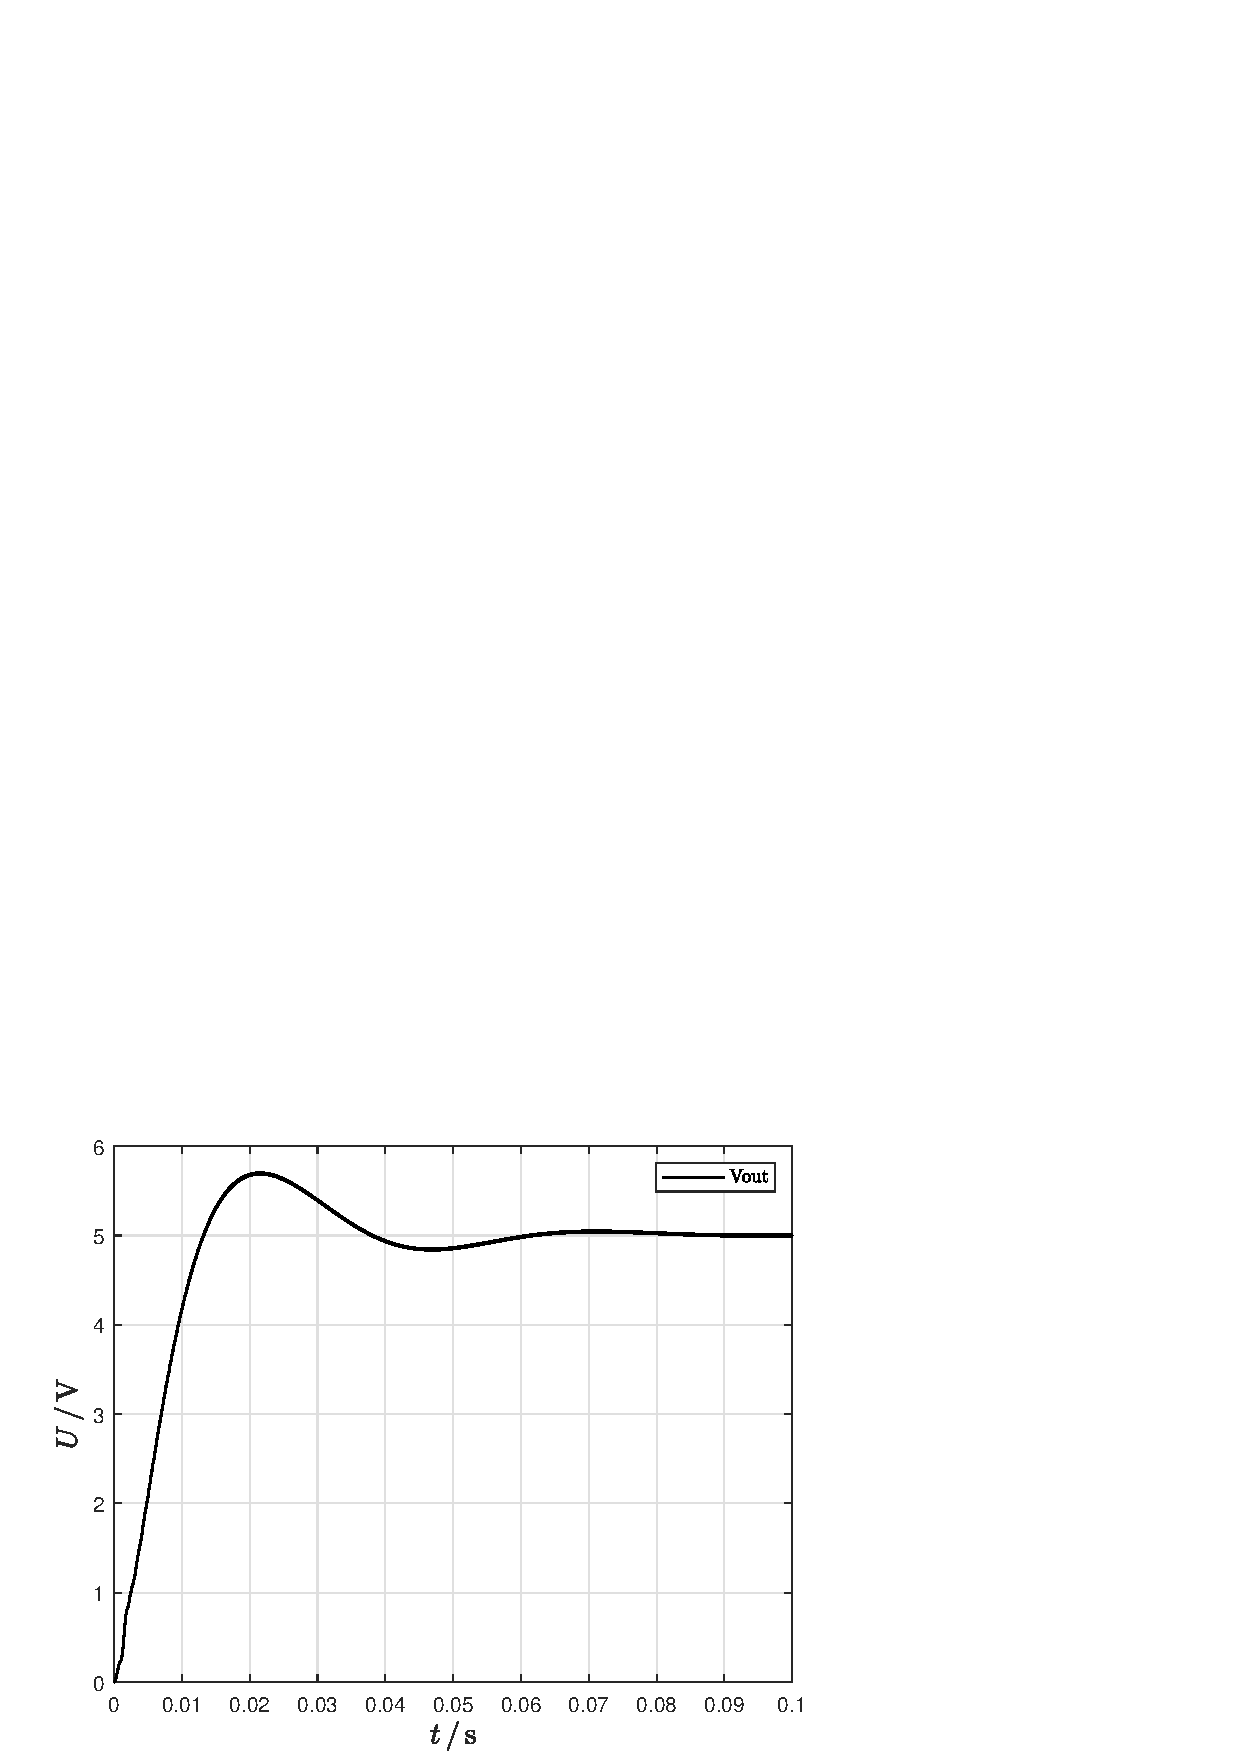
\includegraphics[width=0.8\linewidth]{Figure/Soft.png}
    \caption{FFT LTC3639 mit Filter}
    \label{fig:Soft}
\end{figure}

\begin{figure}[H]
    \centering
    \includegraphics[width=0.8\linewidth]{Figure/ControllerSoft.png}
    \caption{FFT LTC3639 mit Filter}
    \label{fig:ControllerSoft}
\end{figure}

\begin{figure}[H]
    \centering
    \includegraphics[width=0.8\linewidth]{Figure/SystemSoft.png}
    \caption{FFT LTC3639 mit Filter}
    \label{fig:SystemSoft}
\end{figure}


\subsection{PID Auslegung}

\begin{figure}[H]
    \centering
    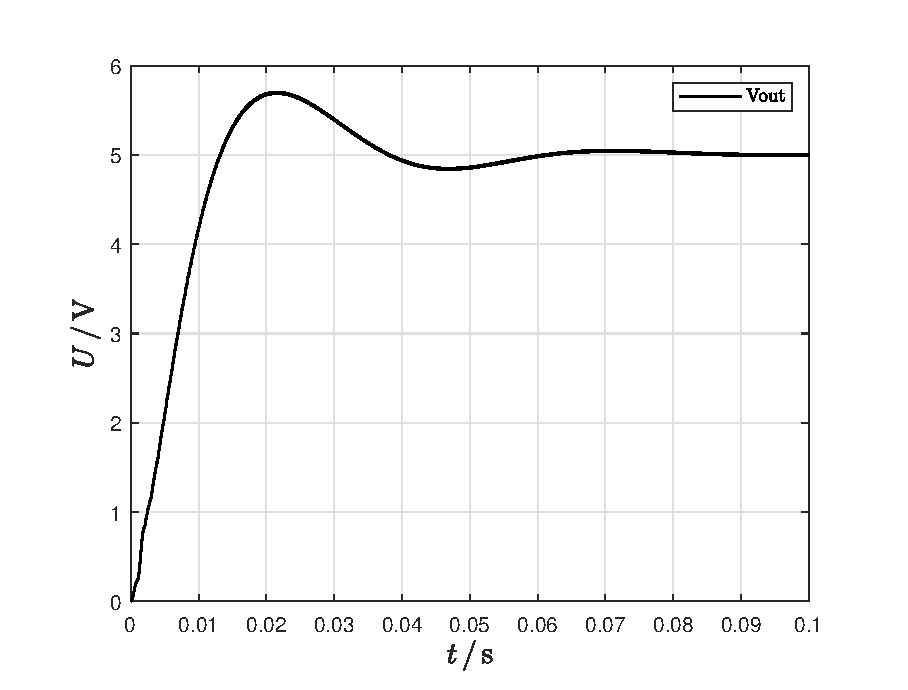
\includegraphics[width=0.8\linewidth]{Figure/Soft.eps}
    \caption{FFT LTC3639 mit Filter}
    \label{fig:SystemSoft}
\end{figure}